\chapter{System Description}
\section{System Model}
\subsection{Overview}
This protocol is typically used under the scenario that there is no reliable or stable networks existed between communication entities (called Alice and Bob). Entities under such conditions can be abstracted as off-line entities in the sense that their network is restricted and can not reach the others' networks. This system allows those off-line entities to communicate by using a Courier to deliver the message. Assuming Alice wants to send a message to Bob, the Courier firstly gets the message from Alice and stores it, then physically transport to Bob and send the message to Bob. \par
The goal of this protocol is to ensure the message from Alice to Bob is secure in the sense that no one can reveal its content but Bob. To achieve that, the Courier should never be trusted, which means the real content of the message should not be accessed by Courier and both Alice and Bob are able to deny the communication with Courier at any time. Furthermore, to prevent sensitive information from being leaked by malicious message recipient (Bob), message creator (Alice) should be able to deny the message content as well.

\subsection{Initial Set-ups}
According to the description above, totally 3 different types of entities are defined in the protocol - Alice, Bob and Courier. Following specification lists the notations and jobs of all 3 entities together with the information they should hold before running the protocol:

\begin{itemize}
\item Alice $\mathcal{A}$ denotes a set of devices who create the message and waits it to be delivered, so it is also called ``message creator". It possesses an unique $\mathcal{ID} \in \{0, 1\}^*$, a secret key $sk_A$ as part of its asymmetric key pair, and the message $\mathcal{M}$ to be sent. \\
$\mathcal{A}$'s ID and public key should be known by at least one Courier so that it will be connected by Courier.

\item Bob $\mathcal{B}$ denotes a set of devices who wait incoming messages delivered by Courier, so it is also called ``message recipient". It possesses an unique $\mathcal{ID} \in \{0, 1\}^*$, and a secret key $sk_B$ as part of its asymmetric key pair.\\
Similarly, its ID and public key should also be known by at least one Courier.

\item Courier $\mathcal{C}$ denotes a set of devices who carry the message of Alice, physically transport from Alice to Bob, and deliver the message to Bob. Initially it only possesses an unique $\mathcal{ID} \in \{0, 1\}^*$ and at least a contact $\mathcal{ID} \in \{0, 1\}^*$ and its corresponding public key, specifies the entity it is going to contact.\\
However, a single Courier will play two different roles in the protocol run - one receives message from Alice, one delivers message to Bob. They are denoted as $\mathcal{CR}$ (Courier Receiver) and $\mathcal{CS}$ (Courier Sender) in the protocol specification. In addition to $\mathcal{CR}$, $\mathcal{CS}$ possesses some more information: the $\mathcal{ID}$ of the message creator and the encrypted message received from $\mathcal{A}$.
\end{itemize}

\paragraph{Public Key Distribution}
The distribution of asymmetric key pairs used for authentication is out of the scope of this protocol, thus $\mathcal{A}$ and $\mathcal{B}$ are assumed to hold their asymmetric key pairs before running the protocol. Furthermore, all entities in the system are assumed to know each other's public key (does not matter it is distributed with manufacture, authenticated by CA, or by key exchange), before running the protocol.

\paragraph{Devices v.s. Entities}
A device $x$ denotes a physical object that runs the protocol. Differently, an entity denotes a particular role in the running of the protocol. It should be noted that any  device can run multiple instances of this protocol with other devices simultaneously, thus a single device can be any three entities at the same time. The role it plays in different communications is defined by what information $x$ holds and what sub-protocol it runs (will be described in Communication Model). However, an entity in the protocol can be associated with only one device.

\subsection{Communication Model}
Ultimately, every single run of this protocol achieves an abstract M-to-1 communication - a certain number of devices $a_0, a_1, ... a_M \in \mathcal{A}$ send message to a single device $b \in \mathcal{B}$ independently, using a device $c \in \mathcal{C}$ as media. As physical transportation is extremely slow and costly compare to network communication, the total number of physical transportation should be reduced to minimum. The optimized solution appeared to be separating the protocol into two main phases - Message Acquisition phase and Message Delivery phase. Assume off-line devices $a_1, a_2, ... a_M \in \mathcal{A}$ need to send message to the off-line device $b \in \mathcal{B}$. In Message Acquisition phase, a Courier will physically transport to every $a \in \mathcal{A}$, connect to it and get the message that is for the $b$. After the Courier collects all needed messages, it enters Message Delivery phase, where the Courier transports to $b$ and transmit all acquired messages to it.

According to explanation above, the whole task can be divided into M + 1 individual communications. Every such individual communication happens between a Courier $c \in \mathcal{C}$ and one of $\mathcal{A} \cup \mathcal{B}$ after the Courier connects to the target. All these communications use one of typical network communication methods (e.g. cable, Wifi, Bluetooth, etc.) and apply its corresponding communication protocols (e.g. TCP/IP, UDP, Bluetooth protocol, etc.). The following figure shows how the communication is organized.

\begin{figure}[h!]
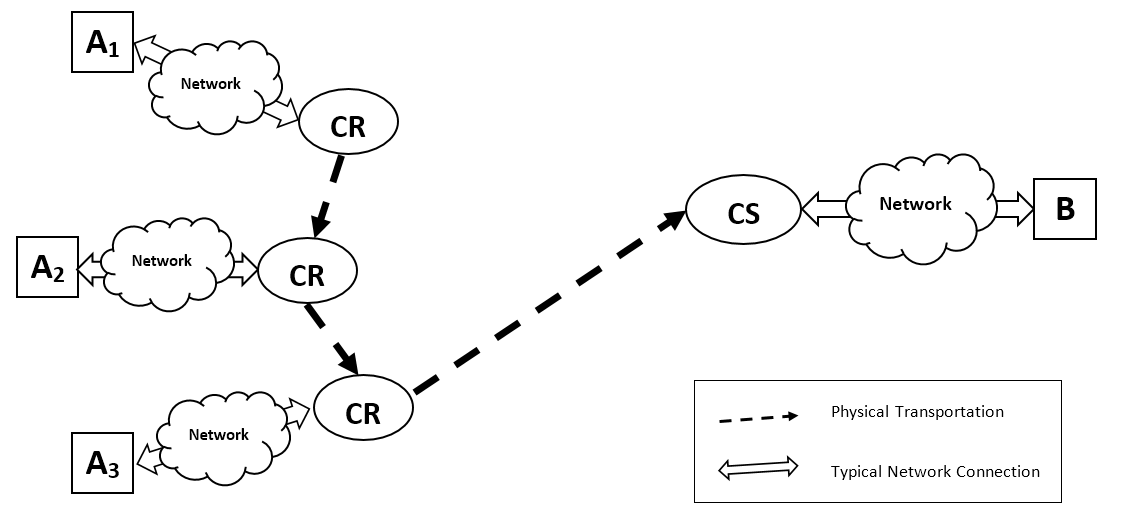
\includegraphics[width=\textwidth,natwidth=1123,natheight=530]{figures/communicationmodel.png}
\caption{Communication Model}
\end{figure}

The figure "Communication Model" illustrates the procedure of a 3-to-1 communication. The Courier first connects to A$_1$, be the role of $\mathcal{CR}$, and gets A$_1$'s message for B through the connection, then disconnects and transports to A$_2$. It should do the same thing to A$_2$ and then transport to A$_3$. After it collects all data from A$_1$, A$_2$ and A$_3$, it transports to B and be the role of $\mathcal{CS}$ to send all collected messages to B. The networks between Courier and As or B can be any kind of connection and do not to be the same, as long as both entities accept. 

To define different kinds of communication, this protocol consists of 2 sub-protocols - a) Submit protocol: how message is submitted from $\mathcal{A}$ to $\mathcal{C}$; b) Transmit protocol: after $\mathcal{C}$ gets connected with $\mathcal{B}$, how message is transmitted to $\mathcal{B}$. These two sub-protocols ensure the secure transmission of message from $\mathcal{A}$ to $\mathcal{B}$ and they will be analysed in the later part.

\subsection{Honest Entity Behaviour}
Generally, all 3 entities in this protocol act as devices who possess their own initial information (described above), take $\mathcal{M}$ as input, and output $\mathcal{M'}$. All honest entities in this protocol should follow the following procedure:
\begin{enumerate}
\item If entity is $\mathcal{C}$, initiate the protocol by sending ${\mathcal{M}_0}'$, otherwise ignore this step.
\item Wait for $\mathcal{M}_1$
\item Receive $\mathcal{M}_1$, decrypt all its ciphertexts and reveal their contents if applicable.
\item Check validity of the contents of $\mathcal{M}_1$ (e.g. check message format, check sender ID, receiver ID, digital signature or MAC, if applicable). If any check violates, immediately report ``Protocol Error" and abort the session.
\item Process the message content (e.g. print the result, stores the contents in local storage).
\item Prepare and send message ${\mathcal{M}_1}'$. If no message to send, abort the session silently.
\item Back to step 2.
\end{enumerate}

However, three entities have different behaviour patterns, they will be specified here, respectively:
\paragraph{Alice $\mathcal{A}$}
\begin{itemize}
\item An entity $a \in \mathcal{A}$ create the message to send, and prepare its meta data. Then it continuously listening to its network, waiting for incoming Couriers.

\item Alice will submit its message to any Courier who request for it. When submitting, the message recipient must be explicitly specified.

\item Alice is allowed to submit any message arbitrary times, to single or multiple Couriers. Alice itself should not care who carries the message, nor how many Couriers carry the message.

\item During an uncompleted session, if no response from Courier for a long time, Alice should be able to detect the timeout, cancel the effects of previous actions in this session and abort the session voluntarily.

\item If the message is not successfully sent, Alice should wait for next Couriers to send this message.
\end{itemize}

\paragraph{Bob $\mathcal{B}$}
\begin{itemize}
\item An entity $b \in \mathcal{B}$ must be continuously listening to its network, waiting for incoming messages.

\item Bob will download all messages from any Courier who transmits. If any message from $\mathcal{A}$ is invalid, Bob simply discards it.

\item Bob will discard all duplicated messages. Duplicated message are defined as messages whose Meta Signature are exactly the same. Because message Meta contains its creator ID and timestamp, same Meta reflects those messages are created by the same entity at the exact same time.

\item During an uncompleted session, if no response from Courier for a long time, Bob should be able to detect the timeout, cancel the effects of previous actions in this session and abort the session voluntarily.
\end{itemize}

\paragraph{Courier $\mathcal{C}$}
\begin{itemize}
\item As Courier's physical transportation is a very complicated task, it is out of the scope of this protocol. It is assumed that Courier is carried by an intelligent agent (such like human) who always knows where the Courier should transport to.

\item Courier should transport to every $a \in \mathcal{A}$ one by one and get their messages if there are any. Courier should be capable of storing those data for a long time.

\item After collect messages from all $a$ in the list, Courier should transport to every $b$ that is the recipient of the Courier and deliver all messages to them. If the receipt from $b$ violates the messages Courier just sent, Courier should resend the messages by restart the session again.

\item Once a full protocol run has been completed, all relative data stored in Courier is expired and should not affect future run of protocol.
\end{itemize}

\section{Adversary Model}
The adversary model in this protocol is mostly derived from Dolev-Yao model which implies ``adversary carries the message" \cite{Dolev}. Moreover, the adversary can also do something special in this protocol system. Specifically, adversary $\mathcal{Z}$ has following capabilities:
\begin{itemize}
\item It supervises the whole network system, which means it knows when, where and how any two entities are communicating, and it knows which entity possesses what information.
\item It can access/rewrite any message passing through the network.
\item It is a legitimate user of the network and it can be any of 3 entities in this protocol.
\item It can access to all the Courier's data at any stage of the protocol.
\item Any $a \in \mathcal{A}$ or $b \in \mathcal{B}$ will always have the opportunity to be connected by any $c \in \mathcal{C}$, which means an adversary will always have opportunity to be contacted by any honest entities.
\end{itemize}

It should be noted that this protocol, same as all other network protocols, is vulnerable to DoS attacks. $\mathcal{Z}$ can always prevent a message from being sent, thus it will not be covered in the security analysis.